% enable this to activate the version for PRINT
% disable this to make the pdf symmetric and without white pages
% => asymmetric alternating left/right margins
% \newcommand*{\printversion}{}%

%% | ---------------- document meta information --------------- |

\newcommand{\Author}{John Smith}
\newcommand{\Department}{Department of Cybernetics}
\newcommand{\Supervisor}{Ing. My Supervisor, Ph.D.}
\newcommand{\SupervisorSpecialist}{Ing. My Specialist, Ph.D.}
\newcommand{\Programme}{Electrical Engineering and Information Technology}
\newcommand{\Field}{Artificial Intelligence and Biocybernetics}
\newcommand{\Title}{My Thesis Title\\[0.5em]Can Span Multiple Lines}
\newcommand{\Keywords}{Unmanned Aerial Vehicles, Automatic Control}
\newcommand{\KlicovaSlova}{Bezpilotní Prostředky, Automatické Řízení}
\newcommand{\Year}{2021}
\newcommand{\Month}{January}
\newcommand{\Date}{\Month~\Year}
\newcommand{\Location}{Prague}

%% | ---------------------- configuration --------------------- |

% most of the configuration stuff happens here
%!TEX root = ../main.tex

%% | ----------------------- page setup ----------------------- |

% define documentclass based on the print/screen version of the document
\pdfoutput=1
\ifdefined\printversion
  \documentclass[a4paper,11pt,twoside,openright]{book}
\else
  \documentclass[a4paper,11pt,twoside,openany]{book}
\fi

% define how "clearpage" works with the print/screen version of the document
\newcommand{\conditionalClearPage}{
  \ifdefined\printversion
    \cleardoublepage
  \else
    \clearpage
  \fi
}

%% | ----------------- commonly used packages ----------------- |

\usepackage[english]{babel}
\usepackage[utf8]{inputenc}
\usepackage{csquotes}
\usepackage{amsmath,amsfonts,amssymb,bm}
\usepackage{nicefrac}
\usepackage{algorithm,algpseudocode}
\usepackage[title,titletoc]{appendix}
\usepackage{latexsym}
\usepackage{a4wide}
\usepackage{color}
\usepackage{indentfirst}
\usepackage{graphicx}
\usepackage{fancyhdr,lastpage}
\usepackage{longtable}
\usepackage{pifont}
\usepackage{makeidx}
\usepackage{multirow}
\usepackage{dcolumn}
\usepackage{epstopdf}
\usepackage{url}
\usepackage{listings}
\usepackage{relsize}
\usepackage{pdfpages}
\usepackage{url}
\usepackage{lipsum}
\usepackage{isotope}
\usepackage{verbatim}
\usepackage{xcolor}
\usepackage{tcolorbox}
\usepackage[colorlinks]{hyperref}
\usepackage{multicol}
\usepackage{subfig}
\usepackage[export]{adjustbox}

% print version has different margins to accommodate the spine of the book
% do not move this around, or it stops working
\ifdefined\printversion
  \usepackage[a4paper,margin=3.2cm,inner=3.4cm,outer=2.0cm]{geometry}
\else
  \usepackage[a4paper,margin=3.2cm,inner=2.7cm,outer=2.7cm]{geometry}
\fi

\hyphenation{}

%% | --------------------- custom commands -------------------- |

\definecolor{cvutblue}{cmyk}{1, 0.43, 0, 0}

% set itemize: bullets type and color
\renewcommand{\labelitemi}{\textcolor{cvutblue}{\raisebox{.45ex}{\rule{.8ex}{.8ex}}}}
\renewcommand{\labelitemii}{\textcolor{cvutblue}{\raisebox{.45ex}{\rule{.8ex}{.8ex}}}}
\renewcommand{\labelitemiii}{\textcolor{cvutblue}{\raisebox{.45ex}{\rule{.8ex}{.8ex}}}}
\renewcommand{\labelitemiv}{\textcolor{cvutblue}{\raisebox{.45ex}{\rule{.8ex}{.8ex}}}}


%% | ---------------------- abbreviations --------------------- |

\usepackage[printonlyused]{acronym}

% use to change margins around abbreviations block
\def\changemargin#1#2{\list{}{\rightmargin#2\leftmargin#1}\item[]}
\let\endchangemargin=\endlist

%% | -------------------- hyper links setup ------------------- |
\hypersetup{
  linkcolor=black,
  anchorcolor=black,
  citecolor=cvutblue,
  filecolor=black,
  menucolor=black,
  runcolor=black,
  urlcolor=cvutblue
}


%% | -------------------------- tikz -------------------------- |

\usepackage{tikz}
\usepackage{pgfplots}
\pgfplotsset{compat=1.14}
\usetikzlibrary{backgrounds,arrows,automata,shapes,positioning,calc,through,spy,shapes,shapes.geometric,shapes.multipart,fit,patterns,fadings}
\pgfdeclarelayer{background}
\pgfdeclarelayer{foreground}
\pgfsetlayers{background,main,foreground}

%% | ------------ siunitx for units of measurements ----------- |

\usepackage{siunitx}
\DeclareSIUnit \parsec {pc}
\DeclareSIUnit \electronvolt {eV}
\DeclareSIUnit \pixel {px}
\DeclareSIUnit \arcmin {arcmin}
\DeclareSIUnit \erg {erg}
\DeclareSIUnit \joul {J}

%% | --------------- change formatting of lists --------------- |

\usepackage{enumitem}
\setlist{nosep}

\renewcommand{\labelenumi}{(\roman{enumi})}

%% | -------------------- table of contents ------------------- |

\usepackage[subfigure]{tocloft}

\tocloftpagestyle{plain}

%% | ----------------- formatting of a chapter ---------------- |

\usepackage{titlesec}

\titleformat{\chapter}[hang]{}{\color{cvutblue}\rule[-0.03cm]{0.50cm}{0.50cm}}{3.2\parskip}{\normalfont\bfseries\LARGE\thechapter\hspace{0.5cm}}
\titlespacing*{\chapter}{0pt}{-1em}{1.5em}

%% | ----------------- formatting of a section ---------------- |

\titleformat{\section}[hang]{}{\hspace{0.11cm}\color{cvutblue}\rule[-0.02cm]{0.30cm}{0.30cm}}{3.7\parskip}{\normalfont\bfseries\large\thesection\hspace{0.5cm}}
\titlespacing*{\section}{0pt}{1em}{0.5em}

\titleformat{name=\section,numberless}[block]
{\normalfont\large\bfseries}{}{0pt}{\large}
% {?}{before}{after}
\titlespacing*{name=\section,numberless}{0pt}{-1em}{2em}

%% | --------------- formatting of a subsection --------------- |

\titleformat{\subsection}[hang]{}{\hspace{0.16cm}\color{cvutblue}\rule[0.03cm]{0.20cm}{0.20cm}}{4.0\parskip}{\normalfont\bfseries\normalsize}
\titlespacing*{\subsection}{0pt}{1em}{0.5em}



%% | ------------------------ biblatex ------------------------ |

\usepackage[backend=bibtex,defernumbers=true,style=ieee,sorting=ydnt,sortcites=true]{biblatex}

% define the source file with bibliography
\addbibresource{main.bib}

\renewcommand*{\bibfont}{\Font}

% add suffix "a" to publications containing the keyword "mine"
% add suffix "c" to publications containing the keyword "mine" && "core"
\DeclareFieldFormat{labelnumber}{%
  \ifkeyword{mine}
    {\ifkeyword{core}
      {{\number\numexpr#1}c}%
      {{\number\numexpr#1}a}%
    }%
    {#1}%
}

\DeclareCiteCommand{\tabcite}%[\mkbibbrackets]
  {\usebibmacro{cite:init}%
   \usebibmacro{prenote}}
  {\usebibmacro{citeindex}%
   \usebibmacro{cite:comp}}
  {}
  {\usebibmacro{cite:dump}%
   \usebibmacro{postnote}}

% define fullciteinbox command
\definecolor{light-gray}{gray}{0.95}
\newcommand{\fullciteinbox}[2]{%

\DeclareCiteCommand{\fullcite}
{\usebibmacro{prenote}}
{\clearfield{addendum}%
  \usedriver
  {\defcounter{minnames}{6}%
  \defcounter{maxnames}{6}}
{\thefield{entrytype}}}
{\multicitedelim}
{\usebibmacro{postnote}}

\begin{tcolorbox}[width=\textwidth,colback={light-gray},title={}]%
\ifx&#2&
\else
  \textbf{#2}:\\\\
\fi
\begin{minipage}[t]{0.07\linewidth}%
\raggedright%
\cite{#1}%
\end{minipage}%
\begin{minipage}[t]{0.93\linewidth}%
\fullcite{#1}%
\end{minipage}%
\end{tcolorbox}%
%}%
\vspace{-0.3em}
}%

% change the bibliography font style
% does not compile without this
\let\bibfont\small

% this is used to print citations of author's work
\defbibenvironment{mycitations}
{\itemize}
{\enditemize}
{\item}

%% | ---------------------- custom macros --------------------- |

\newcommand{\strong}[1]{\textbf{#1}}
\newcommand{\coord}[1]{\textbf{#1}}
\newcommand{\norm}[1]{\left\lvert#1\right\rvert}
\newcommand{\m}[1]{\ensuremath{\mathbf{#1}}}
\newcommand\numberthis{\addtocounter{equation}{1}\tag{\theequation}}
\newcommand{\add}[1]{{\color{green} {#1}}}
\newcommand{\todo}[1]{{\color{red} TODO {#1}}}
\newcommand{\updated}[1]{{\color{blue} {#1}}}
\newcommand{\real}{\mathbb{R}}
\newcommand{\red}[1]{{\color{red} #1}}
\newcommand{\minus}{\scalebox{0.75}[1.0]{$-$}}
\newcommand{\plus}{\scalebox{0.8}[0.8]{$+$}}
\newcommand{\figvspace}{\vspace{-1em}}

% referencing
\newcommand{\reffig}[1]{Fig.~\ref{#1}}
\newcommand{\reflst}[1]{Lst.~\ref{#1}}
\newcommand{\refalg}[1]{Alg.~\ref{#1}}
\newcommand{\refsec}[1]{Sec.~\ref{#1}}
\newcommand{\reftab}[1]{Table~\ref{#1}}
\newcommand{\refeq}[1]{\eqref{#1}}

%% | ----------------- listings - showing code ---------------- |

\usepackage{listings}     
\usepackage{lstautogobble}  % Fix relative indenting
\usepackage{color}          % Code coloring
\usepackage{zi4}            % Nice font

\definecolor{bluekeywords}{rgb}{0.13, 0.13, 1}
\definecolor{greencomments}{rgb}{0, 0.5, 0}
\definecolor{redstrings}{rgb}{0.9, 0, 0}
\definecolor{graynumbers}{rgb}{0.5, 0.5, 0.5}

\usepackage{listings}
\lstset{
    autogobble,
    columns=fullflexible,
    showspaces=false,
    showtabs=false,
    breaklines=true,
    showstringspaces=false,
    breakatwhitespace=true,
    escapeinside={(*@}{@*)},
    commentstyle=\color{greencomments},
    keywordstyle=\color{bluekeywords},
    stringstyle=\color{redstrings},
    numberstyle=\color{graynumbers},
    basicstyle=\ttfamily\footnotesize,
    frame=l,
    framesep=12pt,
    xleftmargin=12pt,
    tabsize=4,
    captionpos=b
}

%% | -------------------- layout parameters ------------------- |

% no indent, free space between paragraphs
\setlength{\parindent}{1cm}
\setlength{\parskip}{1ex plus 0.5ex minus 0.2ex}

% offsets the head down
\setlength{\headheight}{18pt}

% foot line
\renewcommand{\footrulewidth}{0.4pt}

%% | -------------- define the 'full' page style -------------- |

\fancypagestyle{full}{%

  % clear the default layout
  \fancyhead{}
  \fancyfoot{}

  % page header
  \fancyhead[LO]{\leftmark}
  \fancyhead[RE]{\rightmark}
  \fancyhead[LE,RO]{\thepage/\pageref{LastPage}}

  % page footer
  \fancyfoot[L]{CTU in Prague}
  \fancyfoot[R]{\Department}
  \fancyfoot[C]{}
}

%% | -------------- define the 'plain' page style ------------- |

\fancypagestyle{plain}{%

  % clear the default layout
  \fancyhead{}
  \fancyfoot{}

  % page header
  \fancyhead[LE,RO]{\thepage}
}

%% | -------------- Adjust style of chapter names ------------- |

\renewcommand{\chaptermark}[1]{\markboth{\MakeUppercase{\thechapter.\ #1}}{}}

%% | -------- European layout, no extra space after '.' ------- |

\frenchspacing

%% | ----------- adjust the style of the first page ----------- |

\makeatletter
\renewcommand\chapter{\if@openright\cleardoublepage\else\clearpage\fi
                    \thispagestyle{full}% original style: plain
                    \global\@topnum\z@
                    \@afterindentfalse
                    \secdef\@chapter\@schapter}
\makeatother


%% | ---------------------- the contents ---------------------- |

\begin{document}

% this will prevent unwanted line overflows
% http://latexref.xyz/_005cfussy-_0026-_005csloppy.html
\sloppy

\pagenumbering{roman}

%% --------------------------------------------------------------
%% |                         Title page                         |
%% --------------------------------------------------------------

%!TEX root = ../main.tex

\begin{titlepage}
  \begin{center}

    \textsc{\Large Czech Technical University in Prague}\\[1em]
    \textsc{\large Faculty of Electrical Engineering\\
    \Department\\
    Multi-robot Systems\\[3em]
    }
    
\includegraphics[height=4.1cm]{fig/ctu_lion.pdf}\\[3em]

    \textbf{\textsc{\Huge \Title}}\\[2em]

    \textbf{\Large Bachelor's Thesis}\\[6em]

    \textbf{\huge \Author}\\[6em]

    {\large \Location, \Date}\\[3em]

    Study programme: \Programme\\
    Branch of study: \Field\\[4em]

    \textbf{Supervisor: \Supervisor}\\

    \vspace{2pt}

  \end{center}
\end{titlepage}


% set up the page style for the "intro" pages
\pagestyle{plain}

%% --------------------------------------------------------------
%% |                       Acknowledgments                      |
%% --------------------------------------------------------------

\conditionalClearPage

%!TEX root = ../main.tex

\section*{Acknowledgments}

I would like to express my sincere gratitude to my supervisor, Ing. Jan Šedivý, CSc., for his invaluable advice and unwavering support throughout the past year.
His guidance and expertise were instrumental in the completion of this research.

I am also deeply grateful to my colleague, Bc. Adam Jirkovský, for his significant contribution to this research.
Adam's expertise and the code he developed played a crucial role in making this work possible.

Furthermore, I extend my heartfelt thanks to my family: Inessa Davtyan, Inna Zviazdova, Maryia Zviazdova, Natalia Pankova, and Viachaslau Zviazdou.
Their unwavering moral and financial support, along with their constant encouragement, were a source of strength throughout my academic journey.

Finally, I would like to thank my friends, Vsevolod Tiemnohorov, Viachaslau Radzeuski, and Stsiapan Belaushka, for their unwavering support during this challenging yet rewarding experience.

\vspace{2.5cm}


%% --------------------------------------------------------------
%% |                         Assignment                         |
%% --------------------------------------------------------------

\conditionalClearPage

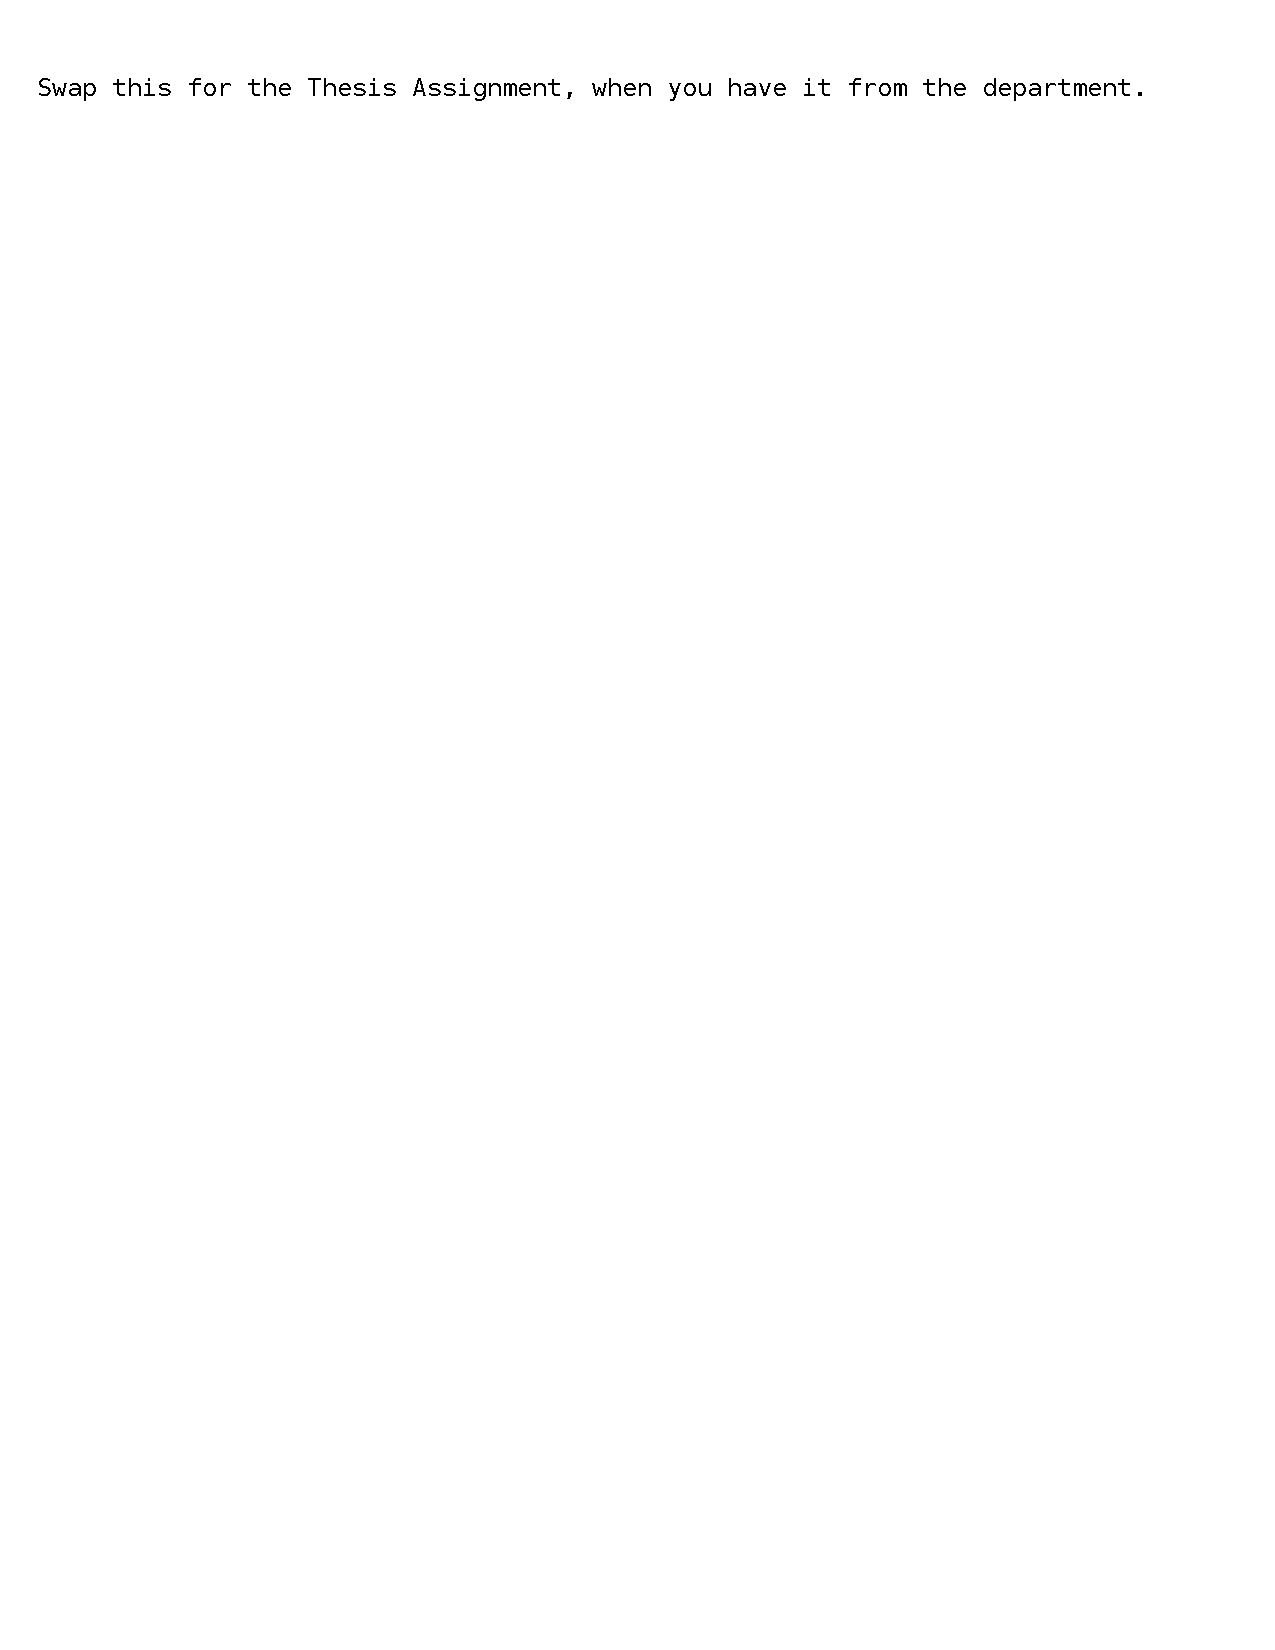
\includepdf{src/assignment.pdf}

%% --------------------------------------------------------------
%% |                         Declaration                        |
%% --------------------------------------------------------------

\conditionalClearPage

~\vfill{}

\section*{Declaration}

I declare that presented work was developed independently, and that I have listed all sources of information used within, in accordance with the Methodical instructions for ob-serving ethical principles in preparation of university theses.
I acknowledge the use of AI tools for rephrasing and grammatical correction.


\vspace{1.5cm}
~\\

In Prague 24.05.2024              \hfill{}                               Yauheni Zviazdou

\hfill{}~~~~~~~~~~~~~~~

\newpage{}


%% --------------------------------------------------------------
%% |                          Abstracts                         |
%% --------------------------------------------------------------

\conditionalClearPage

%!TEX root = ../main.tex

\begin{changemargin}{0.8cm}{0.8cm}

~\vfill{}

\section*{Abstract}
\vskip 0.5em

%The study of autonomous \acp{UAV} has become a prominent sub-field of mobile robotics.
This is en abstract.


\vskip 1em

{\bf Keywords} \Keywords

\vskip 2.5cm

\end{changemargin}


\conditionalClearPage

%!TEX root = ../main.tex

\begin{changemargin}{0.8cm}{0.8cm}

~\vfill{}

\section*{Abstrakt}
\vskip 0.5em

\sloppy
Výzkum na poli autonomních bezpilotních prostředků (UAV) se stal významným oborem mobilní robotiky.

\vskip 1em

{\bf Klíčová slova} \KlicovaSlova

\vskip 2.5cm

\end{changemargin}


%% --------------------------------------------------------------
%% |                        Abbreviations                       |
%% --------------------------------------------------------------

\conditionalClearPage

\begin{changemargin}{0.8cm}{0.8cm}

~\vfill{}

\section*{Abbreviations}

% this will print only the used abbreviations
%!TEX root = ../main.tex

\begin{acronym}
  \acro{CTU}[CTU]{Czech Technical University}
  \acro{API}[API]{Application Programming Interface}
  \acro{RAG}[RAG]{Retrieval-Augmented Generation}
  \acro{NLP}[NLP]{Natural Language Procession}
  \acro{STS}[STS]{Semantic Textual Similarity}
  \acro{QA}[QA]{Question Answering}
  \acro{BERT}[BERT]{Bidirectional Encoder Representations from Transformers}
  \acro{CBOW}[CBOW]{Continuous Bag-of-Words}
  \acro{GloVe}[GloVe]{Global vectors}
  \acro{ML}[ML]{Machine Learning}
  \acro{NN}[NN]{Neural Network}
  \acro{BoW}[BoW]{Bag-of-Words}
  \acro{TF-IDF}[TF-IDF]{Term Frequency-Inverse Document Frequency}
  \acro{OOV}[OOV]{Out of vocabulary}
\end{acronym}


\vskip 2.5cm

\end{changemargin}

\conditionalClearPage

%% --------------------------------------------------------------
%% |                      Table of contents                     |
%% --------------------------------------------------------------

\tableofcontents

\conditionalClearPage

% set up the full page style with normal page numbering
\pagestyle{full}
\pagenumbering{arabic}

%% --------------------------------------------------------------
%% |                        introduction                        |
%% --------------------------------------------------------------

%!TEX root = ../main.tex

\chapter{Introduction\label{chap:introduction}}

\section{Text representation}
The human language, with its nuances and complexities, presents a significant challenge for machines to understand.
\ac{NLP} bridges this gap, and at its core lies the critical concept of text representation.
This process acts as a translator, bridging the gap between the richness of text and the numerical language that machines understand.
By effectively capturing the meaning within words and their relationships, text representation empowers \ac{NLP} models to leverage machine learning's capabilities.
From sentiment analysis to machine translation, this ability to represent meaning fuels the advancements in \ac{NLP}, enabling machines to interact with and decipher human language with ever-increasing accuracy.

\section{Evolution of text representation methods}

\ac{NLP} has undergone a significant transformation in its approach to text representation.
Early methods, such as one-hot encoding, while simple to implement, suffered from limitations in efficiency due to dimensionality and sparsity issues.

Word embedding techniques (e.g., Word2Vec, \ac{GloVe}, FastText) offered a significant improvement by capturing semantic relationships between words through high-dimensional word vectors.
However, these techniques primarily focused on local context within a limited window, hindering their ability to capture complex relationships within sentences or documents.

The emergence of deep learning architectures, particularly transformer-based models like \ac{BERT}, revolutionized the field of text representation.
These models allows to not only understand the meaning of individual words but also consider their interaction and context within a sentence or document.

\begin{figure}
  \centering
  \begin{tikzpicture}
    %Nodes
    \begin{scope}[every node/.style={rectangle, draw=black, thick, align=left, minimum width=10em}]
    \node (Word2Vec)     []                  {Word2Vec};
    \node (GloVe)        [below=of Word2Vec] {\ac{GloVe}};
    \node (FastText)     [below=of GloVe]    {FastText};
    \node (Transformers) [below=of FastText] {Transformers};
    \end{scope}

    % Text labels (outside nodes)
    \node[right=of Word2Vec.east]     {2013};
    \node[right=of GloVe.east]        {2014};
    \node[right=of FastText.east]     {2016};
    \node[right=of Transformers.east] {2017};

    %Lines
    \draw[->] (Word2Vec.south) -- (GloVe.north);
    \draw[->] (GloVe.south)    -- (FastText.north);
    \draw[->] (FastText.south) -- (Transformers.north);
\end{tikzpicture}  
  \caption{Evolution of the text representation methods.}
  \label{fig:ecolution_text_representation}
\end{figure}

\section{Research objective}

This research aims to evaluate the effectiveness of various word, sentence, and paragraph representations for their subsequent application in \ac{RAG} algorithms, with a specific focus on the domain of technical \ac{QA}.

%% --------------------------------------------------------------
%% |                How to write thesis in LaTeX                |
%% --------------------------------------------------------------

%!TEX root = ../main.tex

\chapter{How to write thesis in LaTeX\label{chap:how_to}}

\section{Versioning with git}

Write the LaTeX in such a way that it could be versioned by git, which will help when collaborating with other people.
This means writing \textbf{one sentence per line}.
Even when you use third-party platforms, such as the OverLeaf, you can still share the repository through Git.

\section{Forming paragraphs}

A paragraph is formed in LaTeX by an uninterrupted block of non-empty lines.
It is recommended to keep a single sentence per line (helps with versioning using git).
A new paragraph is started after an empty line.

This is a new paragraph. It is strongly recommended to \textbf{avoid} the use of the \emph{newline} (\texttt{\textbackslash\textbackslash}) feature of LaTeX for forming paragraphs as it doesn't format the new paragraph properly (no space at beginning of the new paragraph).

\section{Linguistic anti patterns}

\subsection{Narrative}

We recommend to write your thesis in plural form of the first-person narrative in combination with passive tense, e.g.:
\begin{itemize}
  \item We discourage the use of any other form, and/or
  \item any other form is discouraged, but \textbf{not}
  \item {\color{red} I discourage you from using the first-person narrative}.
\end{itemize}
Moreover, avoid \enquote{instructional} or \enquote{teacher}-like style of writing, such as {\color{red} \enquote{Now, we multiply the matrix $\mathbf{A}$ by the scalar $c$ to get the scaled matrix $\mathbf{B}$.}}
A better way of writing the same information would be e.g. \enquote{Now, the scaled matrix $\mathbf{B}$ is obtained by multiplying the matrix $\mathbf{A}$ by the scalar $c$.}


\subsection{Pronouns}

The use of pronouns (it, this, they) is strongly \textbf{discouraged}.
Although, pronouns make it easier for you as a writer to form the flow of the text, pronouns also make it much more difficult for the reader to follow the text.
The reader is forced to retain more of the context to substitute and understand what the author meant.
Moreover, pronouns can easily become vague (there is more than one way how to interpret them) and can become invalid while making editorial changes to the text, i.e., when moving sentences around.
A technical text should be written in a way that makes it as easy to read and comprehend as possible and as hard to misunderstand or misinterpret as possible at the same time.

\section{Mathematical notation with LaTeX}

Take care to use the correct mathematical symbols and common ways of denoting mathematical concepts.
Use bold fonts to visually distinguish vectors and matrices ($\mathbf{x}$, $\mathbf{A}$) and scalars ($k$, $N$).

\subsection{Common errors}
A frequent error, carried over from programming languages, is using the asterisk symbol ($*$) to denote multiplication.
The asterisk correctly denotes convolution.
Similarly, the cross sign ($\times$) typically denotes the cross product (it can also used for stating dimensions, such as $\SI{10}{\metre} \times \SI{10}{\metre}$) and thus should not be used for scalar multiplication.
In English mathematical notation, \textbf{scalar multiplication is typically not denoted at all}.

This custom may sometimes make it unclear whether a sequence of letters denotes multiplication of several scalars or a multi-letter variable, such as
{\color{red}%
\begin{equation}
  T = T0 + coeff meas,
\end{equation}
where the variables in this hypothetical equation are $T$, $T0$, $coeff$ and $meas$.}
For this reason, \textbf{avoid using multi-letter variable naming} and strive to denote mathematical variables with single letters optionally a with lower or upper index, or other modifiers (\texttt{\textbackslash{}hat}, \texttt{\textbackslash{}bar}, etc.).
The equation above could be modified to be
\begin{equation}
  T = T_0 + cT_{\text{meas}}.
\end{equation}
If the multiplication is still unclear (e.g. when multiplying many single-letter scalars), the \texttt{\textbackslash{}cdot} symbol may be used such as
\begin{equation}
  P\cdot V = n\cdot R\cdot T.
\end{equation}

\subsection{Equations}
Mathematical equations should be numbered and should be a part of a sentence.
For example, a discrete LTI system update is described as
\begin{equation}
  \mathbf{x}_{\left[k+1\right]} = \mathbf{A}\mathbf{x}_{\left[k\right]} + \mathbf{B}\mathbf{u}_{\left[k\right]},
  \label{eq:lti_system}
\end{equation}
where $\mathbf{x}_{\left[k\right]} \in \mathbb{R}^m$ is the state vector at the sample $k$, $\mathbf{u}_{\left[k\right]} \in \mathbb{R}^n$ is the input vector, $\mathbf{A} \in \mathbb{R}^{m \times m}$ is the main system matrix, and $\mathbf{B} \in \mathbb{R}^{m \times n}$ is the system input matrix.
Proper punctuation should be used after the equation, as if it were an ordinary object in the sentence.

Do not put any empty lines before the equation.
If the sentence that the equation is a part of continues after the equation (as is the case here), do not put empty lines after the equation either.
That would create a new paragraph mid-sentence.
{\color{red}
For an example of how not to do it, the equation

\begin{equation}
  \mathrm{\sigma}(x) = \frac{1}{1 + e^{-x}}
\end{equation}

describes the logistic function often used in machine learning.
}
Observe how a new paragraph is created for the equation and then for this block of text (compare with the proper typesetting above).
Not only does this not look correct, it may also cause incorrect page breaking.

\section{Using footnotes}

Do not be afraid to use footnotes for additional information, such as http links\footnote{This repository: \url{https://github.com/ctu-mrs/thesis_template}.}.
We use footnote links whenever we want to \emph{point} to a website, rather then to cite it as a source.
Like with everything, do not overdo it.

\section{Referencing document elements}

LaTeX allows you to dynamically reference to parts of the documents, such as
\begin{itemize}
  \item figures: \reffig{fig:uavs}, Figure\,\ref{fig:uavs},
  \item equations: eq.~\refeq{eq:lti_system}, \refeq{eq:lti_system},
  \item code: \reflst{lst:references},
  \item and any other object that can contain a \texttt{\textbackslash{}label}.
\end{itemize}
Check the section in the \texttt{document\_setup.tex} that contains useful macros for unifying the references:
\begin{lstlisting}[caption={LaTeX macros for referencing to document elements.},label={lst:references}]
  \newcommand{\reffig}[1]{Fig.~\ref{#1}}
  \newcommand{\reflst}[1]{Lst.~\ref{#1}}
  \newcommand{\refalg}[1]{Alg.~\ref{#1}}
  \newcommand{\refsec}[1]{Sec.~\ref{#1}}
  \newcommand{\reftab}[1]{Table~\ref{#1}}
  \newcommand{\refeq}[1]{\eqref{#1}}
\end{lstlisting}

\section{Abbreviations with Acronym}

Abbreviations are handled by the \emph{acronym} package.
Example sentence with abbreviations: ``\ac{UAV} is a flying vehicle that commonly uses \ac{LiDAR} and \ac{GPS} receiver''.
Note that the acronyms are only explained once in the document by default.
It is good practice to re-explain acronyms used both in the abstract and the rest of the document as the abstract is often presented separately.
This can be achieved by resetting the internal status of the acronyms (\enquote{forgetting} that they were explained) using the \texttt{\textbackslash{}acresetall} command after the abstract.
Please, read the documentation\footnote{Acronym package: \url{http://mirrors.ctan.org/macros/latex/contrib/acronym/acronym.pdf}}.

\section{Units of measurements with Siunitx}

Typesetting of units has never been more accessible with the Siunitx package.
Acceleration is measured in \si{\meter\per\second\squared}.
Gravity accelerates objects at a rate $\approx \SI{9.81}{\meter\per\second\squared}$ near the sea level.
You can define your units if you want.

\section{Hyphens and dashes}

Hyphens and dashes are the various form of the symbol \enquote{-} used in many situations.
There are also various ways how to typeset the symbol in LaTeX.
\begin{itemize}
  \item The \emph{hyphen} is used to compound words, e.g., \enquote{the eye-opener}. The hyphen is typeset as a single \emph{minus}/\emph{hyphen} character: \texttt{-}.
  \item The \emph{en-dash} is used to specify ranges of values, e.g., \enquote{between 2--10}. The en-dash is typeset as two consecutive hyphens characters: \texttt{--}.
  \item The \emph{em-dash} is used to separate complex sentences in place of commas, parenthesis and colons --- each with its particular rules. The em-dash is typeset as three consecutive hyphens characters: \texttt{---}.
\end{itemize}
Check the \url{https://www.thepunctuationguide.com/} for all the details.

\section{Double quotation marks}

\enquote{Double quotes} in English are composed of a pair of opening (``) and closing ('') symbols.
The opening symbol is typeset as two backtick characters: \texttt{``} (typically below the \texttt{Esc} key on the English keyboard), and the closing quotes as two apostrophes: \texttt{''}.
The LaTeX engine will convert them automatically to the opening and closing symbols.
A more robust solution is to use the \texttt{csquotes} package and the \texttt{\textbackslash{}enquote} command which also takes care of nested quoting and other peculiarities.

\section{2D Diagrams with Tikz}

\emph{Tikz} is a powerful tool for drawing 2D (and 3D) shapes and diagrams.
Check the documentation and examples: \url{https://www.overleaf.com/learn/latex/TikZ_package}.
The benefit of using \emph{Tikz}, instead of some other third-party drawing program, are:
\begin{itemize}
  \item fonts are the same as in LaTeX,
  \item you can typeset math in LaTeX,
  \item you can use references to other parts of your document,
  \item you can version the image in git,
  \item the images are easily adjustable while editing your document.
\end{itemize}
Check \reffig{fig:pgfplots_diagram} for example.

\begin{figure}[htbp]
  \centering

  \begin{adjustbox}{max totalsize={0.6\textwidth}{0.90\textheight}, center}
    \tikzset{
  >=stealth',
  punkt/.style={
    rectangle,
    rounded corners,
    draw=black, very thick,
    text width=5.7em,
    minimum height=2em,
    text centered,
  },
  small_punkt/.style={
    rectangle,
    rounded corners,
    draw=black, very thick,
    text width=4.0em,
    text centered,
  },
  arrow/.style={
    ->,
    very thick,
    shorten <=2pt,
    shorten >=2pt,
  },
  arrow_red/.style={
    ->,
    draw=red, very thick,
    shorten <=2pt,
    shorten >=2pt,
  },
}

\begin{tikzpicture}[node distance=1cm, auto,]

  % outer circle nodes
  \node[punkt] (sensor) {Sensor size};
  \node[punkt, inner sep=5pt, below = of sensor, shift = {(-6.0, -0.75)}] (aircraft) {Aircraft\\size};
  \node[punkt, inner sep=5pt, below = of sensor, shift = {(0.0, -4.0)}] (constraints) {Environment constraints};
  \node[punkt, inner sep=5pt, below = of sensor, shift = {(6.0, -0.75)}] (strategy) {Localization strategy};

  % inner circle nodes
  \node[small_punkt, inner sep=5pt, below = of sensor, shift = {(0.0, 0.5)}] (sensor2) {\scriptsize Sensor size};
  \node[small_punkt, inner sep=5pt, right = of aircraft, shift = {(0.5, -0.0)}] (aircraft2) {\scriptsize Aircraft\\size};
  \node[small_punkt, inner sep=5pt, above = of constraints, shift = {(0.0, -0.5)}] (constraints2) {\scriptsize Environment\\constraints};
  \node[small_punkt, inner sep=5pt, left = of strategy, shift = {(-0.5, -0.0)}] (strategy2) {\scriptsize Localization\\strategy};

  \path[->] ($(sensor.west)+(0, 0)$) edge [arrow,bend right=45] ($(aircraft.north)$);
  \path[->] ($(aircraft.south)+(0, 0)$) edge [arrow,bend right=45] ($(constraints.west)$);
  \path[->] ($(constraints.east)+(0, 0)$) edge [arrow,bend right=45] ($(strategy.south)$);
  \path[->] ($(strategy.north)+(0, 0)$) edge [arrow,bend right=45] ($(sensor.east)$);

  % inner circle paths
  \path[->] ($(sensor2.west)+(0, 0)$) edge [arrow_red, bend right=45, dashed] ($(aircraft2.north)+(0.0, 0.0)$);
  \path[->] ($(aircraft2.south)+(0, 0)$) edge [arrow_red, bend right=45, dashed] ($(constraints2.west)+(0.0, 0.0)$);
  \path[->] ($(constraints2.east)+(0, 0)$) edge [arrow_red, bend right=45, dashed] ($(strategy2.south)+(0.0, 0.0)$);
  \path[->] ($(strategy2.north)+(0, 0)$) edge [arrow_red, bend right=45, dashed] ($(sensor2.east)+(0.0, 0.0)$);

  % outer inner arrows
  \draw [->] ($(sensor.south)+(0, 0)$) -- ($(sensor2.north)$) node [midway, shift = {(0.0, 0.0em)}] {smaller};
  \draw [->] ($(aircraft.east)+(0, 0)$) -- ($(aircraft2.west)+(0.0, 0.0)$) node [midway, shift = {(0.0, 0.0em)}] {smaller};
  \draw [->] ($(constraints.north)+(0, 0)$) -- ($(constraints2.south)+(0.0, 0.0)$) node [midway, shift = {(0.0, 0.0em)}] {more complex};
  \draw [->] ($(strategy.west)+(0, 0)$) -- ($(strategy2.east)+(0.0, 0.0)$) node [midway, shift = {(0.0, 0.0em)}] {smarter};

\end{tikzpicture}

  \end{adjustbox}

  \caption{Example of a 2D diagram using tikz \emph{PGFPlots}.}
  \label{fig:pgfplots_diagram}
\end{figure}

\section{Data plots with PGFPlots}

\emph{PGFPlots} produces nice 2D and 3D data plots from data stored in CSV.
The plot parameters can be versioned and easily adjusted by editing the plot definition file.
\begin{itemize}
  \item Documentation and manual: \url{https://ctan.org/pkg/pgfplots}
  \item Compile the plots individually and then include the pdfs because it can take longer.
  \item Example located in \texttt{fig/plots/example\_plot}, see \reffig{fig:pgfplots_data}.
  \item You could include the latex file directly. However, it will take longer to compile, and platforms such as Overleaf can have a problem with that.
\end{itemize}

\begin{figure}[htbp]
  \centering
  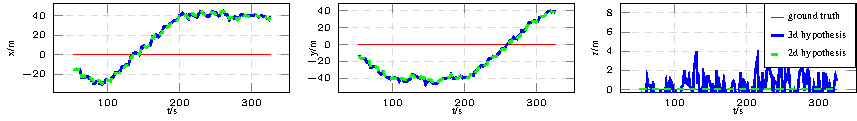
\includegraphics[width=1.0\textwidth]{./fig/plots/example_plot/hypotheses.pdf}
  \caption{Example of a 2D plot using \emph{PGFPlots}.}
  \label{fig:pgfplots_data}
\end{figure}

\section{3D Plots with Sketch}

\emph{Sketch} is a tool for defining a 3D scene using simple descriptive language.
The 3D scene is then converted to \emph{Tikz}, which is later compiled to pdf.
The benefits of using \emph{Sketch} are similar to using \emph{Tikz}: LaTeX fonts, versioning using git, and cleanness of the result.
See the example image in \reffig{fig:coordinate_systems}.
\begin{itemize}
  \item Documentation and manual: \url{http://www.frontiernet.net/~eugene.ressler/}
  \item Cross-compilation from \emph{Sketch} to \emph{pdf} using the \texttt{fig/sketch/compile\_sketch.sh} script.
\end{itemize}

\begin{figure}[htbp]
  \centering
  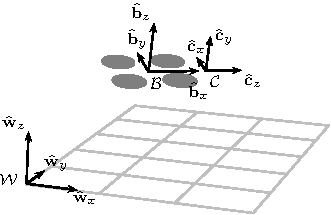
\includegraphics[width=0.4\textwidth]{./fig/sketch/coordinate_frames.pdf}
  \caption{Depiction of the used coordinate systems. The image was drawn using \emph{Sketch}.}
  \label{fig:coordinate_systems}
\end{figure}

\section{Image collages with Subfig}

We recommend using the \texttt{subfig} package, which provides the \texttt{\textbackslash{}subfloat} command.
It is more versatile than the simpler \texttt{subcaption} package.
Check \reffig{fig:uavs} for an example.

\begin{figure}[htbp]
  \centering
  \subfloat[A UAV, the T650 model.] {
    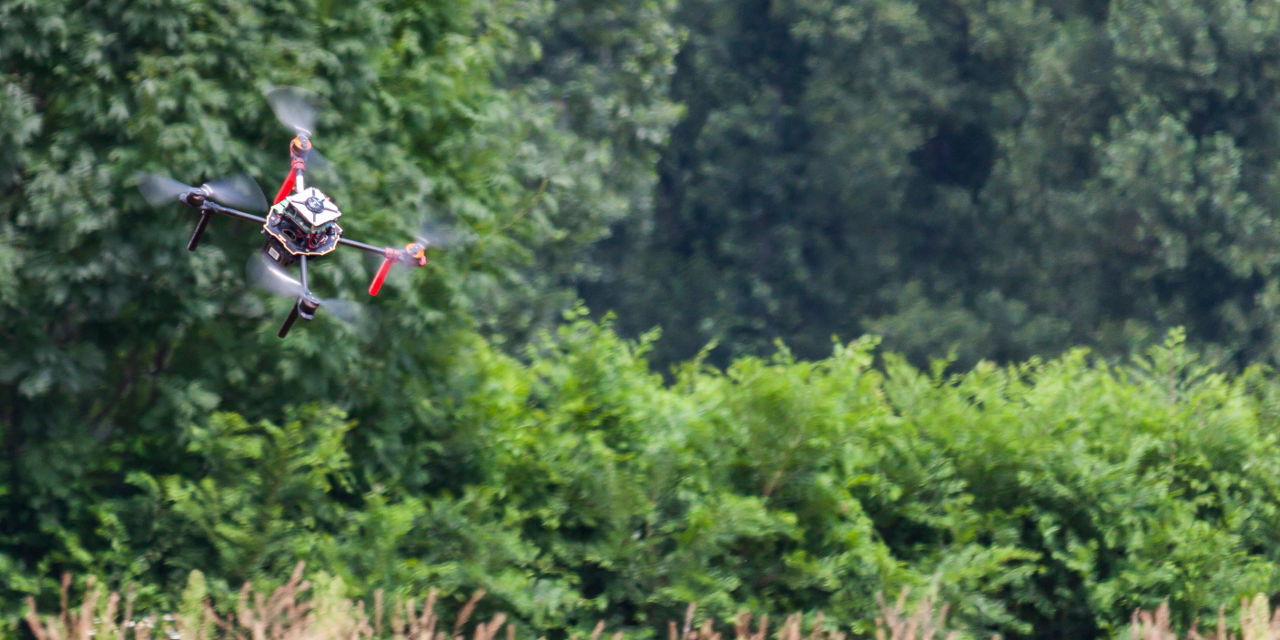
\includegraphics[width=0.48\textwidth]{./fig/photos/uav1.jpg}
    \label{fig:uavs_1}
  }
  \subfloat[Another UAV, again, the T650 model.] {
    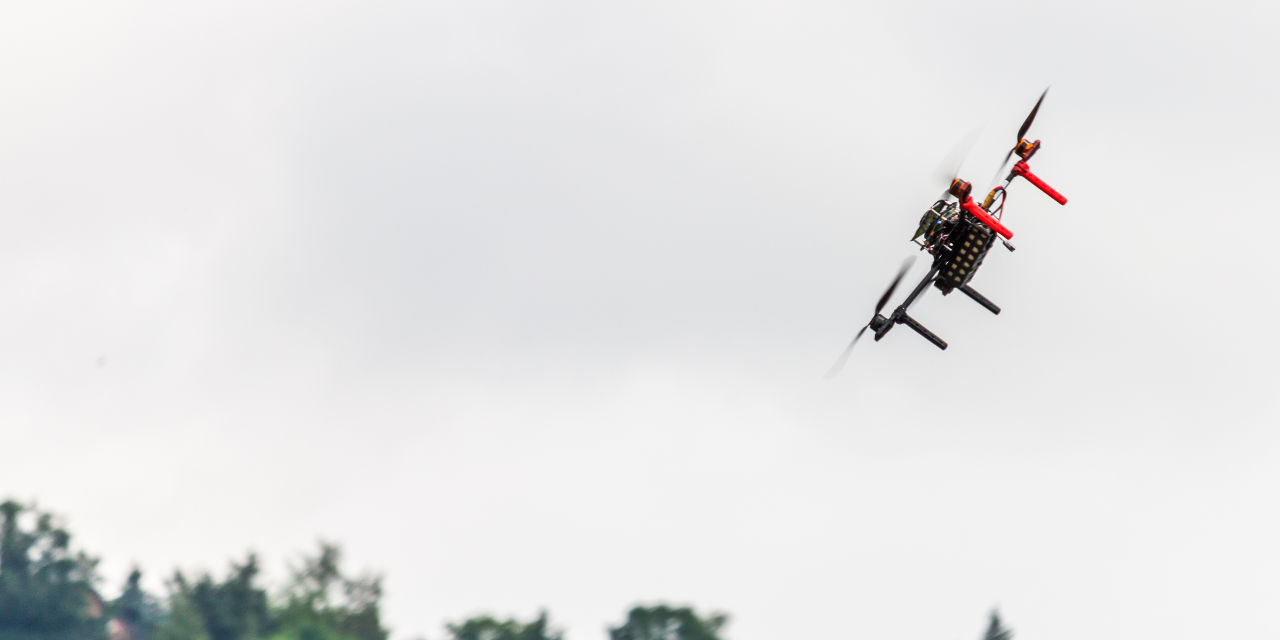
\includegraphics[width=0.48\textwidth]{./fig/photos/uav2.jpg}
    \label{fig:uavs_2}
  }
  \caption{
The caption should mention both subfigures, the \reffig{fig:uavs_1} and the \reffig{fig:uavs_2}.
You can just refer to them as (a) and (b) in the main Figure's caption, but beware, you need to keep it correct as you edit.
}
  \label{fig:uavs}
\end{figure}

\section{Citations with Biblatex}

\emph{Biblatex} is probably the most powerful citation package for LaTeX.
It consumes the standard \texttt{.bib} file. However, it can sort and filter the citations using the \texttt{keywords} tag.
Citing references is done using the \texttt{cite} command, e.g., \cite{baca2021mrs}.
You can also define some nice citation boxes, such as this one:
\fullciteinbox{baca2021mrs}{}

\section{Image overlays with Tikz}

\emph{Tikz} is very useful to create custom image overlays.
The overlay can be set such that the image is spanned by Cartesian coordinates $\left(x, y\right) \in \left[0, 1\right]^2$
Example can be seen in \reffig{fig:tikz_overlay}.

\begin{figure}[!t]

  \centering

  \subfloat {\begin{tikzpicture}
    \node[anchor=south west,inner sep=0] (a) at (0,0) { 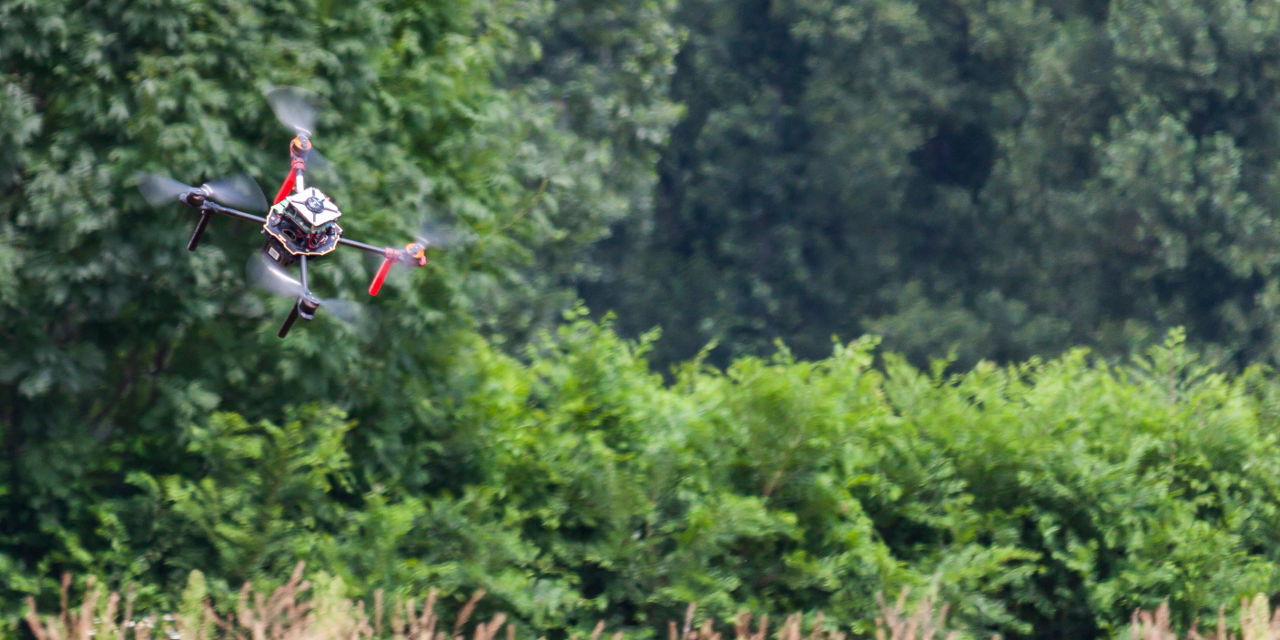
\includegraphics[width=0.45\textwidth]{./fig/photos/uav1.jpg}};
    \begin{scope}[x={(a.south east)},y={(a.north west)}]

      %%{ grid for placing the elements

      % % useful grid to help you find coordinates for plotting the overlay
      % \draw[black, xstep=.1, ystep=.1] (0,0) grid (1,1);
      % \foreach \i in {0,0.1,0.2,0.3,0.4,0.5,0.6,0.7,0.8,0.9,1} {
      %   \node[align=center] at (\i, -0.05) {\i};
      %   \node[align=center] at (\i, 1.05) {\i};
      %   \node[align=center] at (-0.05, \i) {\i};
      %   \node[align=center] at (1.05, \i) {\i};
      % }

      %%}

      % plot some stuff over the image

      % plot white background behind the letter (a)
      \fill[white] (0.001, 0.001) rectangle (0.08,0.14);

      % plot black border
      \fill[draw=black, draw opacity=0.5, fill opacity=0] (0,0) rectangle (1, 1);

      % write the letter (a) in the bottom-left corner
      \draw (0.04,0.06) node [text=black] {\small (a)};

      % plot black border
      \draw[->, white, thick] (0.50, 0.80) -- (0.30, 0.67);
      \draw (0.50,0.86) node [text=white] {\small \textbf{UAV}};
    \end{scope}
  \end{tikzpicture}}
\hfill%
\subfloat {\begin{tikzpicture}
    \node[anchor=south west,inner sep=0] (a) at (0,0) { 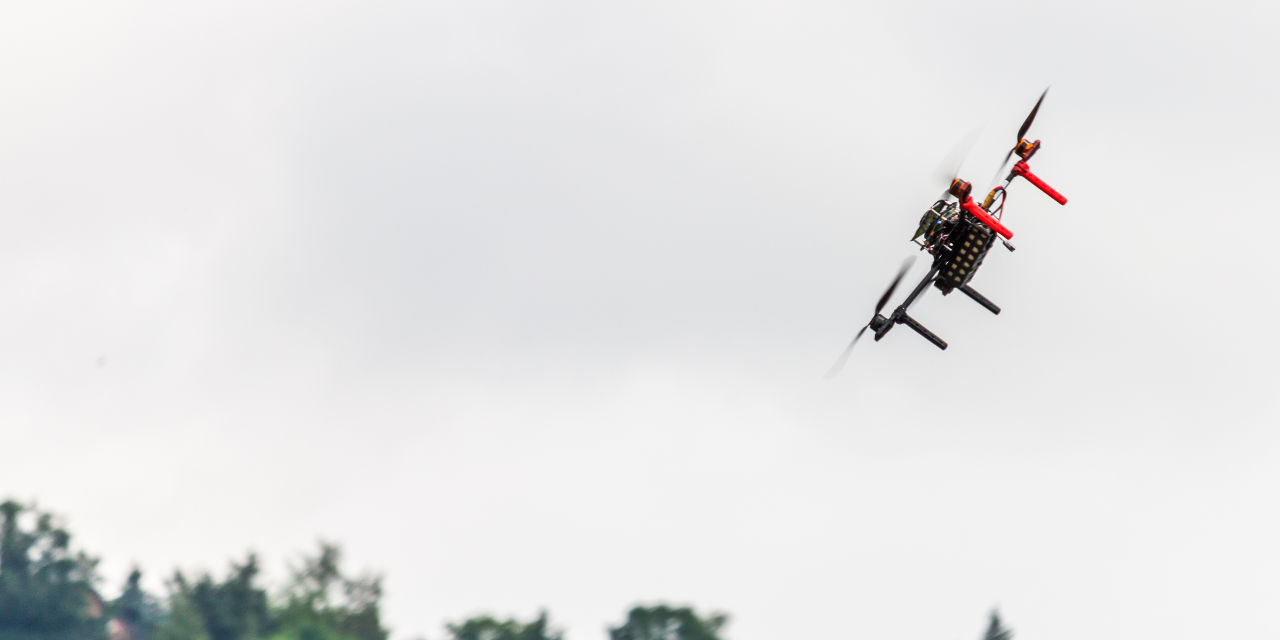
\includegraphics[width=0.45\textwidth]{./fig/photos/uav2.jpg}};
    \begin{scope}[x={(a.south east)},y={(a.north west)}]

      %%{ grid for placing the elements

      % useful grid to help you find coordinates for plotting the overlay
      \draw[black, xstep=.1, ystep=.1] (0,0) grid (1,1);
      \foreach \i in {0,0.1,0.2,0.3,0.4,0.5,0.6,0.7,0.8,0.9,1} {
        \node[align=center] at (\i, -0.05) {\i};
        \node[align=center] at (\i, 1.05) {\i};
        \node[align=center] at (-0.05, \i) {\i};
        \node[align=center] at (1.05, \i) {\i};
      }

      %%}

      % plot some stuff over the image

      % plot white background behind the letter (b)
      \fill[white] (0.001, 0.001) rectangle (0.08,0.14);

      % plot black border
      \fill[draw=black, draw opacity=0.5, fill opacity=0] (0,0) rectangle (1, 1);

      % write the letter (b) in the bottom-left corner
      \draw (0.04,0.06) node [text=black] {\small (b)};
    \end{scope}
  \end{tikzpicture}}


  \caption{Example of using Tikz for image overlays. (a) shows a final product, (b) shows a grid useful for nailing down the coordinates.}
  \label{fig:tikz_overlay}

\end{figure}

\section{General tips}

In general, strive to make the paper easy to read and understand, and hard to misunderstand or misinterpret.
Here are some more specific tips on how to achieve that (and other general suggestions).

\begin{itemize}
  \item
    \textbf{Be consistent.}
    This applies in all contexts.
    For example, if you decide to use the name \enquote{LiDAR}, do not mix it with \enquote{LIDAR} or \enquote{Lidar},
    do not mix different mathematical notations,
    ensure your Figures have the same style and use the same graphics for the same concepts,
    etc.
  \item 
    After you finish writing or modifying any of:
    \begin{itemize}
      \item a sentence,
      \item a paragraph,
      \item a section/chapter,
      \item the whole paper/thesis,
    \end{itemize}
    \textbf{re-read it} to make sure that it makes sense, it is coherent and correct, and doesn't contain typos.
  \item
    If you're using a LLM-based tool (ChatGPT etc.) for grammar-proofing or even formulation of sentences, \textbf{do not just copy-paste its response} to your query.
    The previous rule applies doubly here.
    LLMs tend to often produce confident-sounding nonsense, sentences with reformulated duplicated content, or with a slightly changed meaning.
    They are a good tool to get inspiration to start writing about a subject, for grammar-checking, or for finding alternative, nice-sounding formulations, but they can lie or warp facts --- take care when using them!

\end{itemize}


%% --------------------------------------------------------------
%% |                         Conclusion                         |
%% --------------------------------------------------------------

%!TEX root = ../main.tex

\chapter{Conclusion \label{chap:conclusion}}

This thesis investigated the effectiveness of transformer-based models for text representation compared to traditional methods in the context of semantic similarity assessment for Czech text.

The analysis began with a comprehensive review of traditional text representation methods.
Their architectures, underlying principles, strengths, weaknesses, and specific applications were examined.
This review established a foundation for understanding the evolution of text representation techniques.

Following this, the study shifted its focus to transformer architectures.
Here, the investigation delved into the inner workings of these models and explored their advantages over traditional methods.
The \ac{BERT} model served as a specific example, with an explanation of its training process and its strengths in capturing semantic meaning from textual data.

To ensure objective assessment of model quality for the chosen task, two relevant evaluation methods were reviewed.
These established methods provided a framework for comparing the performance of different text representation models used for semantic similarity assessment in Czech text.

Next, the investigation explored the \ac{RAG} model.
Core concepts, operational principles, and critical parameters influencing \ac{RAG}'s accuracy were examined.
This in-depth analysis proved crucial for effectively configuring and evaluating \ac{RAG} within the context of the chosen task.

Recognizing the importance of language-specific analysis, Czech was chosen as the target language.
The study incorporated both diacritic and diacritic-less text versions to account for potential variations within Czech text data.
The established UPV FAQ benchmark served as the standard for consistent and reliable evaluation.

A baseline performance metric was established using the FastText model.
This baseline provided a benchmark for comparing the performance of the transformer-based models.
Following the establishment of this baseline, a diverse selection of 15 transformer-based model groups (encompassing a total of 37 models) were chosen for further evaluation.

The \ac{RAG} evaluation process involved testing five different chunk sizes.
This exploration aimed to understand the impact of chunk size on both the factuality (accuracy) of retrieved information and computational efficiency (processing time).
The initial stage focused on selecting optimal text representation models.
We employed \ac{GTE}\textsubscript{Small} for embedding generation and GPT-3.5-turbo for answer generation.
GPT-4o was used in a separate process to assess the quality of answers generated by GPT-3.5-turbo.

After we made evaluation of the chosen models to detect best text representation models.
The evaluation results revealed that a significant portion of the transformer-based models outperformed the baseline, suggesting their promise for semantic similarity assessment in Czech text.
A detailed analysis of model performance and influencing factors identified \ac{mE5} \textsubscript{Large} as the top performer.
A confusion matrix visualized its evaluation on a specific benchmark subset.
Additionally, "balanced models" exhibiting the best performance relative to their model size were highlighted.
These included SimCSE-RetroMAE-Small, the small version of \ac{GTE}, and all sizes of \ac{mE5}, demonstrating the potential of both large and efficient models for this task.

The evaluation then proceeded to analyze the impact of chunk size on the \ac{RAG} model itself.
The first stage involved calculating the average time required for embedding generation with different chunk sizes using \ac{GTE}\textsubscript{Small}.
This analysis aimed to identify potential variations in processing time based on chunk size.
The results yielded unexpected findings, which were subsequently interpreted as a potential consequence of improved transformer model parallelism when handling larger sequences of tokens.

Following the analysis of processing time, the study investigated the impact of chunk size on model accuracy.
Based on the evaluation results, a chunk size of 4096 characters was identified as optimal for the \ac{RAG} model.


% \section{CONCLUSION STRUCTURE}
% \begin{itemize}
%     \item Summarize the key takeaways from the research, emphasizing the most effective text representation model for \ac{RAG} in technical \ac{QA} based on the evaluation criteria.
%     \item Briefly mention the trade-offs between factuality, CPU usage, and other factors in selecting representations for \ac{RAG}.
%     \item Suggest potential future research directions, such as exploring other text representation methods or evaluating \ac{RAG} performance on different datasets.
% \end{itemize}


%% --------------------------------------------------------------
%% |                         References                         |
%% --------------------------------------------------------------

\chapter{References}

\printbibliography[heading=none,title={}]

%% --------------------------------------------------------------
%% |                         Appendices                         |
%% --------------------------------------------------------------

\appendix
\renewcommand\chaptername{Appendix}

\renewcommand{\thechapter}{A}
\renewcommand\chaptername{Appendix A}

\chapter{Appendix A}

\end{document}
